\documentclass{llncs}
\usepackage{fullpage}
\usepackage{float}
\usepackage{tikz}
\usepackage{amsmath}
\usetikzlibrary{arrows, automata, positioning}

\usepackage{enumitem}
\usepackage{graphicx}
\usepackage{array}
\usepackage{pgfgantt}
\usepackage{booktabs}
\usepackage{hyperref}
\usepackage[utf8]{inputenc}

% Redefine las subsecciones para usar letras en lugar de números
\usepackage{titlesec}
\renewcommand\thesubsection{\alph{subsection})}

\begin{document}

\title{Toma de decisiones}

\author{Miguel Ángel Dorado Maldonado}
\institute{\email{miguelangeldorado10@uma.es} \\
TCIS. Universidad de Málaga.}

\maketitle

\vspace{1cm}

\section{El dilema del prisionero es uno de los problemas más estudiados a lo largo de la historia. Este problema consiste en lo siguiente:}

\textit{La policía arresta a dos sospechosos. No hay pruebas suficientes para condenarlos y, tras haberlos separado, los visita a cada uno y les ofrece el mismo trato. Si uno confiesa y su cómplice no, el cómplice será condenado a la pena total, diez años, y el primero será liberado. Si uno calla y el cómplice confiesa, el primero recibirá esa pena y será el cómplice quien salga libre. Si ambos confiesan, ambos serán condenados a seis años. Si ambos lo niegan, todo lo que podrán hacer será encerrarlos durante un año por un cargo menor.}

\vspace{0.25cm}
Además, si este problema se repite entre los mismos prisioneros muchas veces se tiene el conocido como Dilema del Prisionero Iterado.

\vspace{0.25cm}
Se pide que responda a las siguientes preguntas:

\begin{enumerate}
	\vspace{0.5cm}
	\item [a)] Realice una tabla con las diferentes combinaciones de años en prisión para uno de los sospechosos.

		\begin{center}
			\begin{tabular}{|c|p{5cm}|p{5cm}|}
				\hline
				& \textbf{P2 Confiesa} & \textbf{P2 No confiesa} \\
				\hline
				\textbf{P1 Confiesa} & 6 años para ambos & P1 queda libre y P2 cumple la pena de 10 años \\
				\hline
				\textbf{P1 No confiesa} & P1 cumple la pena de 10 años y P2 queda libre & 1 año para ambos\\
				\hline
			\end{tabular}
		\end{center}


	\vspace{0.5cm}
	\item [b)] ¿Cuál es la mejor estrategia para ganar el Dilema del Prisionero? Explique por qué.

		\vspace{0.25cm}
		Analicemos los diferentes escenarios posibles:

		\begin{itemize}
			\item Si ambos confiesan, ambos son condenados a 6 años.
			\item Si uno confiesa y el otro no, el que confiesa es liberado y el otro es condenado a 10 años.
			\item Si ninguno confiesa, ambos son condenados a 1 año.
		\end{itemize}

		En caso de confesar, la media de años que pasaría en prisión contemplando las dos posibilidades que mi cómplice elija sería de (6+0)/2 = 3 años de media. En caso de que el cómplice no confiese, me libraría de la cárcel y en caso de que confiese, pasaría 6 años que no llega a ser la pena máxima.

		\vspace{0.25cm}
		En caso de no confesar, la media de años que pasaría en prisión contemplando las dos posibilidades que mi cómplice eleja sería de (10+1)/2 = 5.5 años de media. En caso de que el cómplice no confiese, pasaría 1 año en prisión y en caso de que este confesara, pasaría la pena máxima, 10 años.

		\vspace{0.25cm}
		Se minimizan las pérdidas. Confesando el peor caso posible sería 6 años mientras que no confesando el peor caso posible sería 10 años. Confesando el mejor caso posible sería 0 años mientras que no confesando el mejor caso posible sería 1 año. Por tanto, la mejor estrategia sería confesar, ya que la media de años que pasaría en prisión sería menor que si no confesara.

	\vspace{0.5cm}
	\item [c)] Explique 3 estrategias diferentes para ganar el Dilema del Prisionero Iterado: en qué consisten dichas estrategias y qué objetivo se persigue en cada una de ellas.

		\vspace{0.25cm}
		Existen un gran número de estrategias para ganar el Dilema del Prisionero Iterado. A continuación, se presentan tres de ellas:

		\begin{itemize}
			\item [1.] \textbf{Tit for Tat.} Conocido como toma y daca, consiste en empezar cooperando pero en el momento en el que el otro falle, se copia la opción elegida por él. A largo plazo fomenta la cooperación porque muestra confianza siempre que el oponente colabore y venganza al traicionar
			\item [2.] \textbf{Pavlot.} Cooperar si ambos lo hicieron en la ronda anterior. En caso de perder, cambiar de opción. La estrategia es flexible y permite algo de recuperación tras un error.
			\item [3.] \textbf{Cooperar siempre.} Coopera siempre da igual la elección del oponente. Muy vulnerable a la traición continua. Promueve la cooperación.
		\end{itemize}


	\vspace{0.5cm}
	\item [d)] Comente qué es el Torneo de Axelrod. Incluya una imagen de Robert Axelrod.

	\vspace{0.25cm}
	El torneo de Axelrod es un experimento de la teoría de juegos diseñado por Robert Axelrod en la década de los 80. El objetivo era eplorar como las diferentes estrategias posibles pueden evolucionar con el paso de las iteraciones. Las estrategias competían en una serie de rondas del Dilema del Prisionero Iterado. Se utilizaba un puntaje acumulativo para determinar que estrategia había sido la más exitosa.

	\vspace{0.25cm}
	La estrategia ganadora fue Tit for Tat (toma y daca). Aún tratandose de una estrategia simple, consiguió el primer puesto gracias a fomentar la cooperación y castigar la traición en la siguiente jugada.
	
\end{enumerate}

\begin{figure}[H]
	\begin{center}
		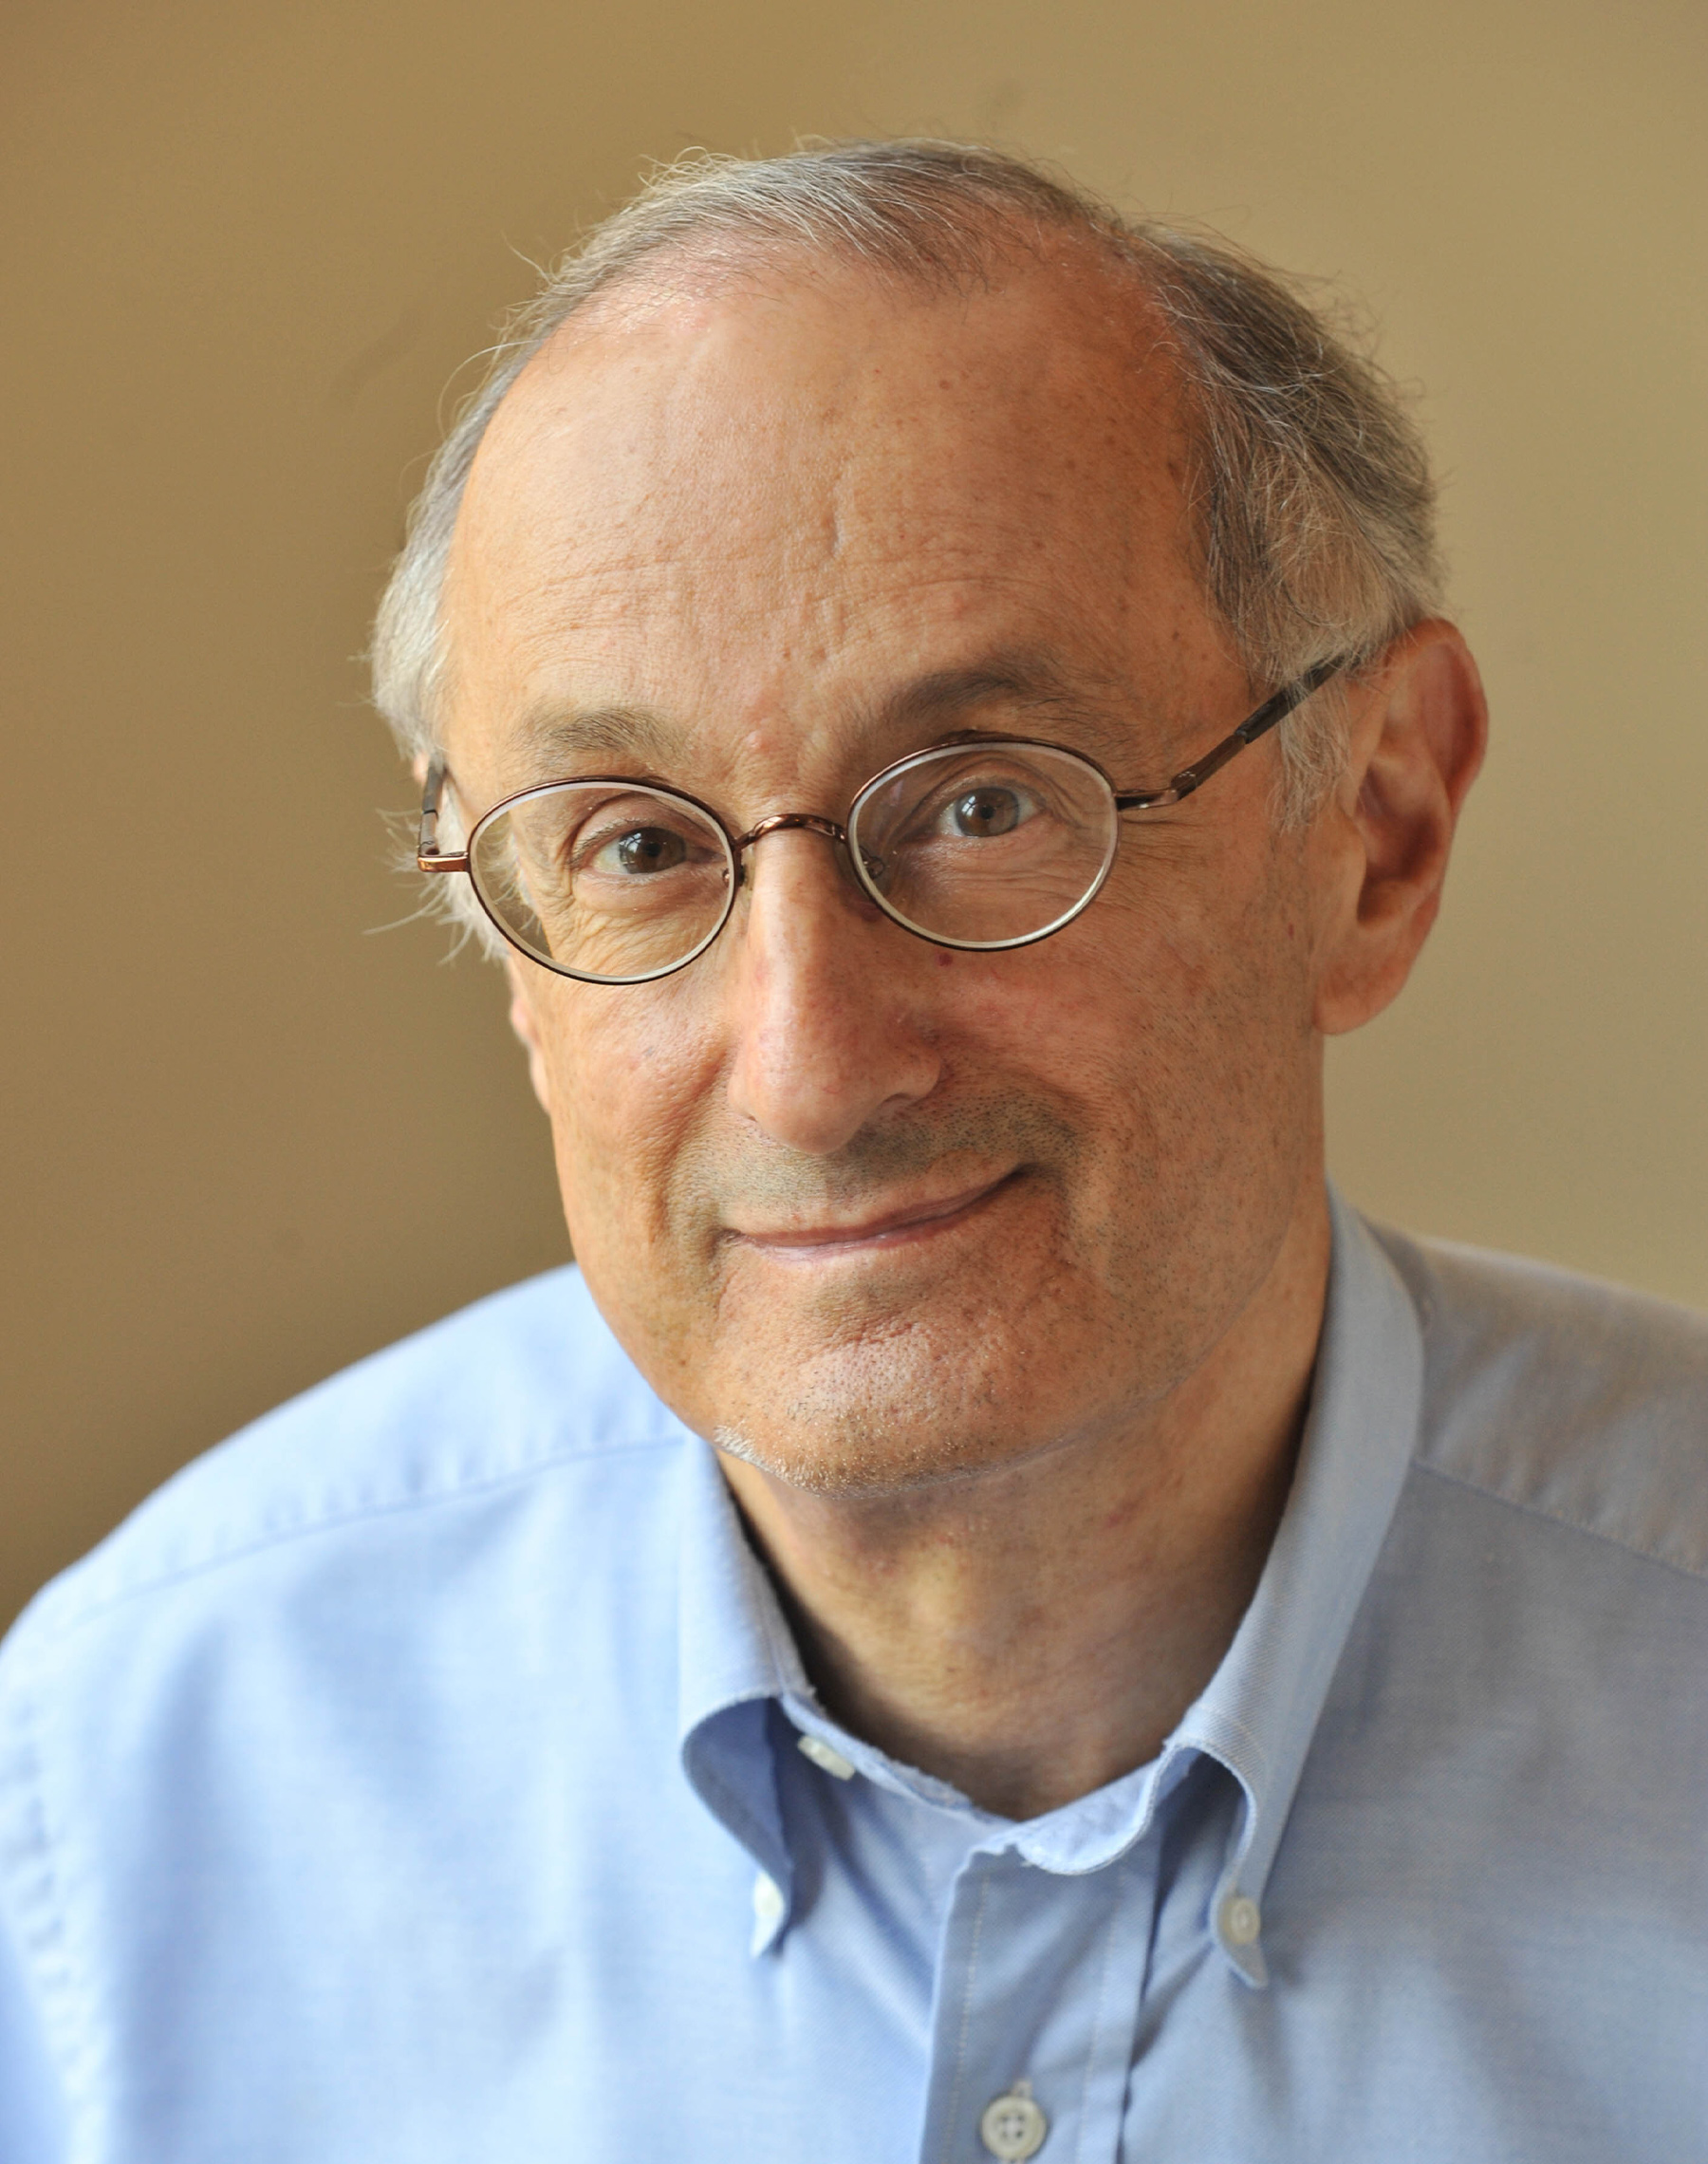
\includegraphics[width=0.3\textwidth]{axelrod.jpg}
		\caption{Robert Marshall Axelrod}
	\end{center}
\end{figure}

\newpage
\section{Se le propone participar en el juego denominado Dados a Seis, con una inscripción de 1€. Este juego consiste en lanzar dos dados distintos. Si la suma de los resultados de los dados es menor a 6 se gana el juego; en caso contrario, se pierde. Si se gana el juego, se obtiene un premio de 1.50€. ¿Jugaría a este juego? ¿Y si el premio fuera de 2€?}

Analizamos estadísticamente si merece la pena jugar.
Partimos de dos dados con números del 1 al 6 cada uno. Esto nos deja con un total de $6^2$ combinaciones totales.

Veamos cuantas combinaciones cumplen con la restricción de suma \le 6

\begin{enumerate}
	\item [-] \textbf{suma 2:} (1,1)
	\item [-] \textbf{suma 3:} (1,2), (2,1)
	\item [-] \textbf{suma 4:} (1,3), (2,2), (3,1)
	\item [-] \textbf{suma 5:} (1,4), (2,3), (3,2), (4,1)
	\item [-] \textbf{suma 6:} (1,5), (2,4), (3,3), (4,2), (5,1)
\end{enumerate}

En total hay 1 + 2 + 3 + 4 + 5 = 15 combinaciones posibles. Por tanto, la probabilidad de ganar es de 15/36 = 0.4167.

\vspace{0.25cm}
Si la incripción es de 1€ y el premio es de 1.50€, en caso de ganar se ganaría 0.5€ y en caso de perder se perdería 1€. La esperanza matemática sería la probabilidad de ganar por dinero ganado menos probabilidad de perder por dinero perdido:

\begin{equation*}
	\text{E} = (\frac{15}{36} \cdot 0.50) + (\frac{21}{36} \cdot -1) = 0.208 - 0.583 = -0.375
\end{equation*}

Obtenemos una esperanza matemática negativa, por lo que no merece la pena jugar.

\vspace{0.25cm}
Si el premio fuera de 2€, en caso de ganar se ganaría 1€ y en caso de perder se perdería 1€. La esperanza matemática sería la probabilidad de ganar por dinero ganado menos probabilidad de perder por dinero perdido:

\begin{equation*}
	\text{E} = (\frac{15}{36} \cdot 1) + (\frac{21}{36} \cdot -1) = 0.417 - 0.583 = -0.166
\end{equation*}

De igual forma, obtenemos una esperanza matemática negativa, por lo que tampoco merece la pena jugar.

\newpage
Yo, Miguel Ángel Dorado Maldonado, a día 23 de diciembre de 2024, declaro bajo mi palabra de honor que el trabajo aquí entregado es de mi autoría y originalidad. Asimismo, confirmo que no he utilizado recursos externos que no hayan sido debidamente citados ni recibido ayuda no autorizada en su realización.

\end{document}
